\section{Choice of Fill Reducing Reordering}
\label{subseq:fill-in-reordering}

Fill reducing reordering is the first and the most important step of sparse matrix decomposition since it has its direct impact on the assembly tree structure. As we mentioned above, the tree structure defines the task parallelism as well as sizes of frontal matrices and thus performance of the method.\\


MUMPS provides various algorithms for reordering described in section \ref{subseq:mumps-review}. A detailed study and comparison between different methods were done by \citeauthor{guermouche2003memory} in work \cite{guermouche2003memory} for sequential execution of the analysis phase. \citeauthor{guermouche2003memory} noticed that the trees generated by METIS and SCOTCH were rather wide (because of the global partitioning performed at the top), while the trees generated by AMD, AMF and PORD tend to be deeper. In addition, they came to two important conclusions. Firstly, they noticed both SCOTCH and METIS generated much better balanced trees in contrast to other methods. Secondly, according to their results, SCOTCH and METIS produced trees with bigger frontal matrices than those generated by the other reorderings \cite{guermouche2003memory}.\\


In this section we are going to investigate influence of two different parallel fill reducing packages, namely: PT-Scotch and ParMETIS, on parallel performance of MUMPS. The algorithmic difference between PT-Scotch and ParMETIS was explained in section \ref{subseq:mumps-review}.\\


To perform a test, the default PETSc, MUMPS, PT-Scotch and ParMETIS libraries were downloaded, compiled, configured and link together. The test was carried out using only flat-MPI mode without explicit process pinning. The results are shown in figure \ref{fig:mumps-ordering-1} as well as in appendix \ref{app:app-fill-reducing-reodering}.\\


\figpointer{\ref{fig:mumps-ordering-1}}
\begin{figure}[htpb]
\centering
	\begin{tabular}{cc}
		\subfloat[k3-18]{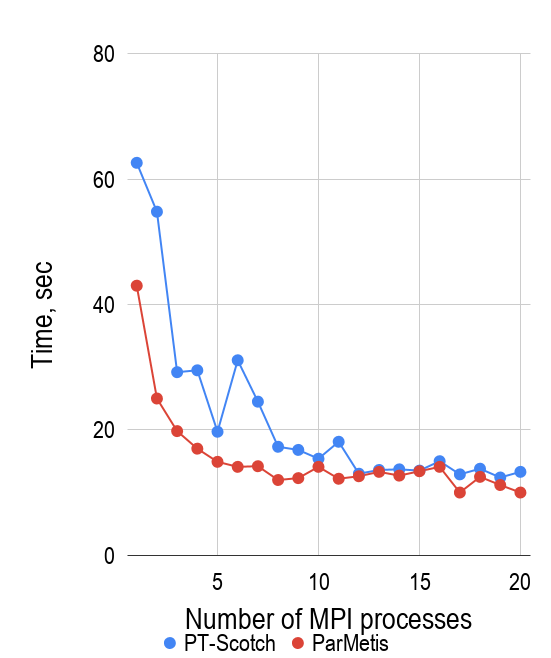
\includegraphics[width=0.48\textwidth]{figures/chapter-2/ordering/k3-18.png}} &
		\subfloat[cube-64]{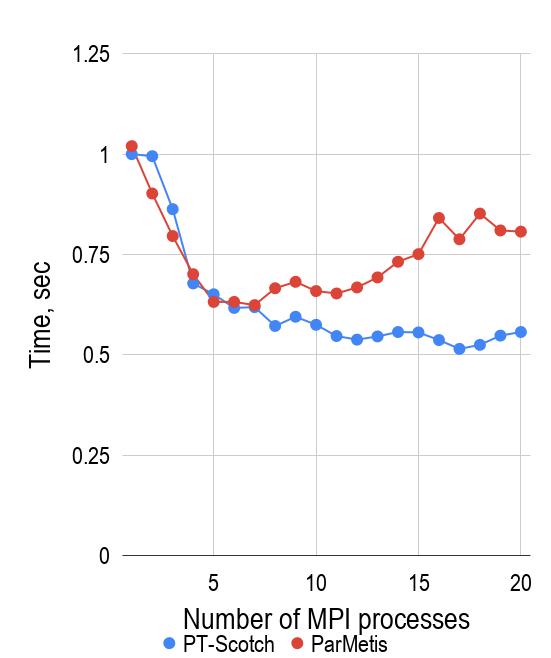
\includegraphics[width=0.48\textwidth]{figures/chapter-2/ordering/cube-64.png}} \\
		\subfloat[pwr-3d]{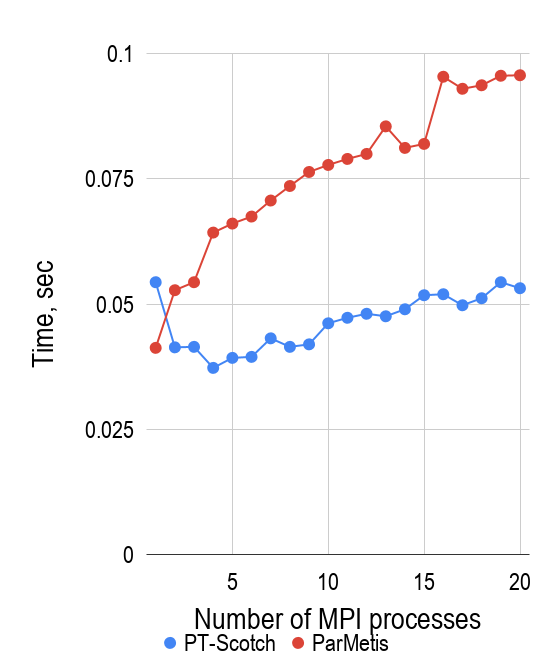
\includegraphics[width=0.48\textwidth]{figures/chapter-2/ordering/pwr-3d.png}} &
		\subfloat[k3-2]{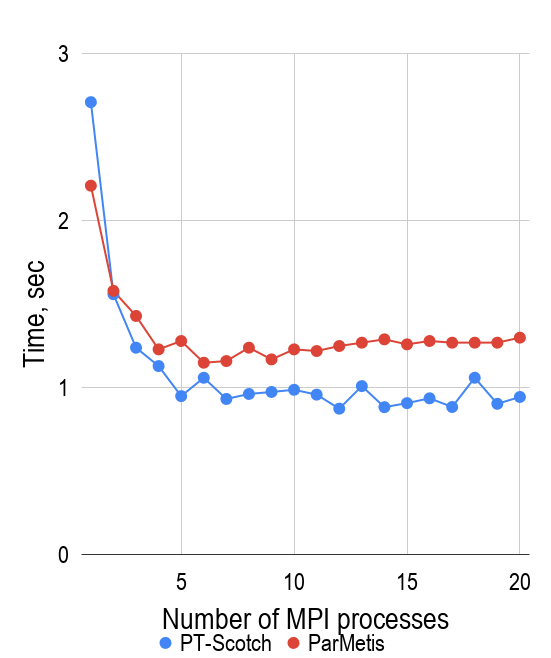
\includegraphics[width=0.48\textwidth]{figures/chapter-2/ordering/k3-2.png}} \\
	\end{tabular}
	\caption{Comparison of different fill-reducing algorithms}
	\label{fig:mumps-ordering-1}
\end{figure}


\todo{rewrite the results}
% Huge difference between different fill reducing schemes
According to the results, parallel performance of MUMPS can vary significantly between the libraries. In average, the difference between different fill-in reducing algorithms can achieve almost BRA\%.\\


It is important to mention that both packages, PT-Scotch and ParMetis, use heuristic approaches with the main aim to reduce fill-in of the factors and thus do not directly consider quality of the resultant elimination tree. It is relevant to assume that efficiency of a particular heuristic can be very sensitive to a matrix structure and size. \todo{insert example of k3-2 and show that expensive reordering can help to get better tree} This fact makes it difficult to predict which algorithm is better to use for a specific case in advance. Taking GRS matrix set as an example, we can observe that PT-Scotch is the best choice for small and medium matrices, namely: \textit{cube-5}, \textit{cube-64}, \textit{k3-2} and \textit{pwr-3d} cases. However, at the same time PerMetis tends to work better for relatively big systems such as \textit{cube-645} and \textit{k3-18}.\\


% profiling of cube-5 and pwr-3d with ParMetis
During the test, application of ParMetis in case of small systems of equations showed a strong negative effect on parallel performance of MUMPS. The execution time for factorization of \textit{pwr-3d} and \textit{cube-5} matrices grew with the increase of processing units (figure \ref{fig:mumps-ordering-matrices-total-time}).\\


\figpointer{\ref{fig:mumps-ordering-matrices-total-time}}
\begin{figure}[htpb]
\centering
	\begin{tabular}{cc}
		\subfloat[pwr-3d]{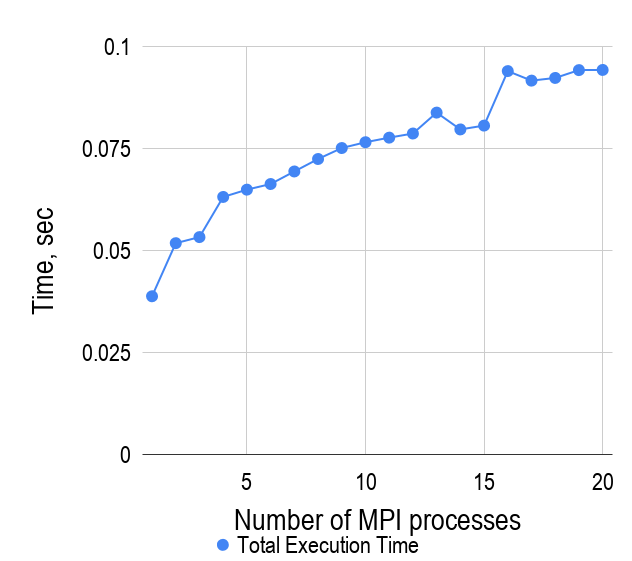
\includegraphics[width=0.475\textwidth]{figures/chapter-2/ordering/profiling/total-time-pwr-3d.png}} &
		\subfloat[cube-5]{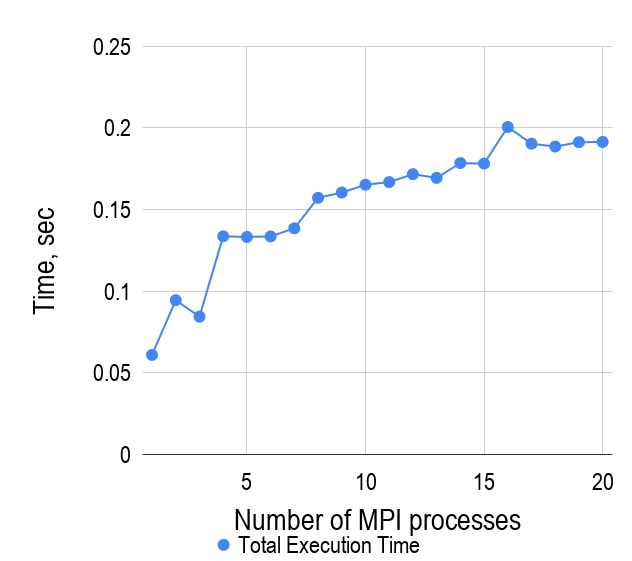
\includegraphics[width=0.475\textwidth]{figures/chapter-2/ordering/profiling/total-time-cube-5.png}} \\
	\end{tabular}
	\caption{MUMPS-ParMetis parallel performance in case of relatively small matrices}
	\label{fig:mumps-ordering-matrices-total-time}
\end{figure}


A simple profiling showed two important things. Firstly, numerical factorization time and time spent on the analysis phase had the same order in case of sequential execution i.e. 1 MPI process. Secondly, while numerical factorization time barely decreased with increase of number of processing elements, time spent on analysis phase time significantly grew. The results of profiling are shown in figure \ref{fig:mumps-ordering-matrices-profiling}.\\


\figpointer{\ref{fig:mumps-ordering-matrices-profiling}}
\begin{figure}[htpb]
\centering
	\begin{tabular}{cc}
		\subfloat[pwr-3d]{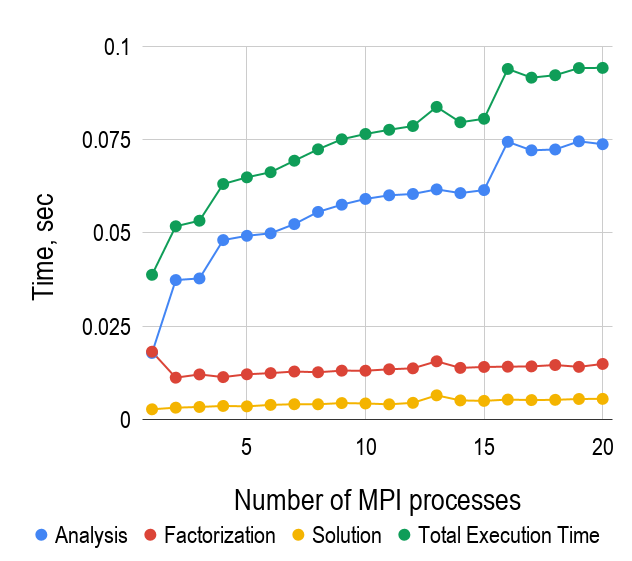
\includegraphics[width=0.475\textwidth]{figures/chapter-2/ordering/profiling/profiling-pwr-3d.png}} &
		\subfloat[cube-5]{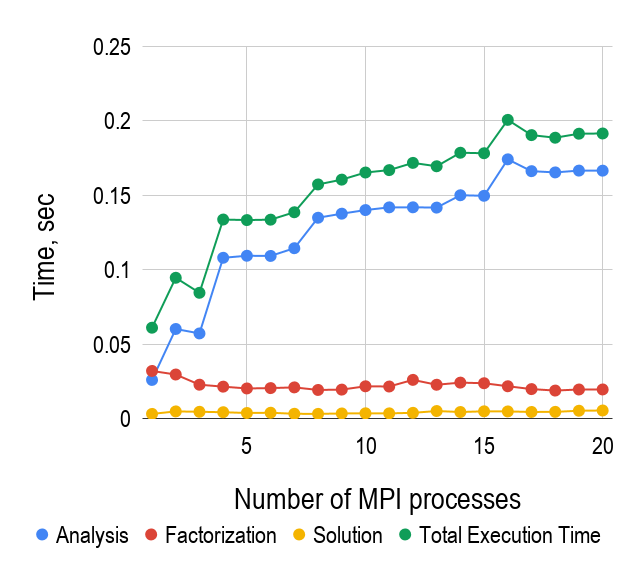
\includegraphics[width=0.475\textwidth]{figures/chapter-2/ordering/profiling/profiling-cube-5.png}} \\
	\end{tabular}
	\caption{Profiling of MUMPS library with using ParMetis as a fill-in reducing algorithm in case of factorization of relatively small matrices}
	\label{fig:mumps-ordering-matrices-profiling}
\end{figure}


In this section, we have presented the influence of different fill-in reducing algorithms on parallel performance of MUMPS. We have observed the right choice of the algorithm can lead to significant improvements in terms of the overall execution time. We have showed there is no a single algorithm that performs the best for all test cases. At the moment of writing, we came to conclusion there was no an indirect metric to predict the best algorithm in advance for a specific system of equations and only a flat-MPI test could be used for that purposed. Sometimes PT-Scotch and ParMetis can perform nearly the same like it is in case of \textit{CurlCurl\_3} and \textit{cant}, for example (see appendix \ref{app:app-fill-reducing-reodering}). Therefore, from time to time, it can be quite difficult to make a decision which package to use. At the end, we have assigned each test case to a specific fill reducing reordering method based on results of the conducted experiments and our subjective opinion. The results are summarized it in tables \ref{table:GRS-ordering-assignment} and \ref{table:SuiteSparse-ordering-assignment}. \\ 



\begin{table}[htpb]
\centering
\begin{tabular}{|c|c|c|c|c|}
\hline
Matrix Name & Ordering  & n       & nnz      & nnz / n \\ \hline
cube-5      & PT-Scotch & 9325    & 117897   & 12.6431 \\ \hline
cube-64     & PT-Scotch & 100657  & 1388993  & 13.7993 \\ \hline
cube-645    & ParMetis  & 1000045 & 13906057 & 13.9054 \\ \hline
k3-2        & PT-Scotch & 130101  & 787997   & 6.0568  \\ \hline
k3-18       & ParMetis  & 1155955 & 7204723  & 6.2327  \\ \hline
pwr-3d      & PT-Scotch & 6009    & 32537    & 5.4147  \\ \hline
\end{tabular}
\caption{GRS matrix set: assignment of matrices to a specific fill-in reducing algorithm based on parallel performance during flat-MPI tests}
\label{table:GRS-ordering-assignment}
\end{table}


\begin{table}[htpb]
\centering
\begin{tabular}{|c|c|c|c|c|}
\hline
Matrix Name & Ordering  & n       & nnz      & nnz / n \\ \hline
cant        & ParMetis  & 62451   & 4007383  & 64.1684 \\ \hline
consph      & PT-Scotch & 83334   & 6010480  & 72.1252 \\ \hline
memchip     & PT-Scotch & 2707524 & 13343948 & 4.9285  \\ \hline
PFlow\_742  & PT-Scotch & 742793  & 37138461 & 49.9984 \\ \hline
pkustk10    & PT-Scotch & 80676   & 4308984  & 53.4110 \\ \hline
torso3      & ParMetis  & 259156  & 4429042  & 17.0903 \\ \hline
x104        & PT-Scotch & 108384  & 8713602  & 80.3956 \\ \hline
CurlCurl\_3 & PT-Scotch & 1219574 & 13544618 & 11.1060 \\ \hline
Geo\_1438   & ParMetis  & 1437960 & 63156690 & 43.9210 \\ \hline
\end{tabular}
\caption{SuiteSparse matrix set: assignment of matrices to a specific fill-in reducing algorithm based on parallel performance during flat-MPI tests}
\label{table:SuiteSparse-ordering-assignment}
\end{table}



From now onwards, we will use this assignment for the rest of the study to keep consistency between tests and show the overall effect of 
\textit{optimal parameters} on the default MUMPS settings at the end. \\